\chapter{Results}

From the data gathered from the measurements a total of 23 datasets with the average of 335 and a total of 7708 trials were used for the analysis. The starting location IDs are identical with the building-IDs inside the unity environment and are not replaced with new numbers for the analysis.

\subsection{Summary statistics of dependent variables}

\begin{enumerate}
	\item \textbf{Absolute angular deviation:} \\
	This variable has the mean of 48.08 with the standard deviation of 44.30, and median of 33.70. (See figure \ref{fig:angular_dev_dists})
	
	\begin{figure}[h]
		\centering
		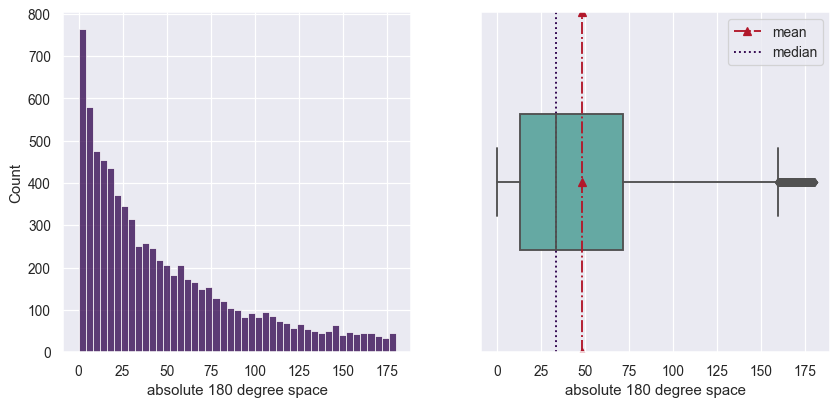
\includegraphics[width=150mm]{figures/angular_deviation_hist_box_23.png}
		\caption[Distribution of the absolute angular deviation]{distribution of the absolute angular deviation}
		\label{fig:angular_dev_dists}
	\end{figure}

	\item \textbf{Reaction times:} \\
	This variable has the mean of 7.77 with the standard deviation of 5.56, and median of 6.06. (See figure \ref{fig:rt_dists})
	
	\begin{figure}[h]
		\centering
		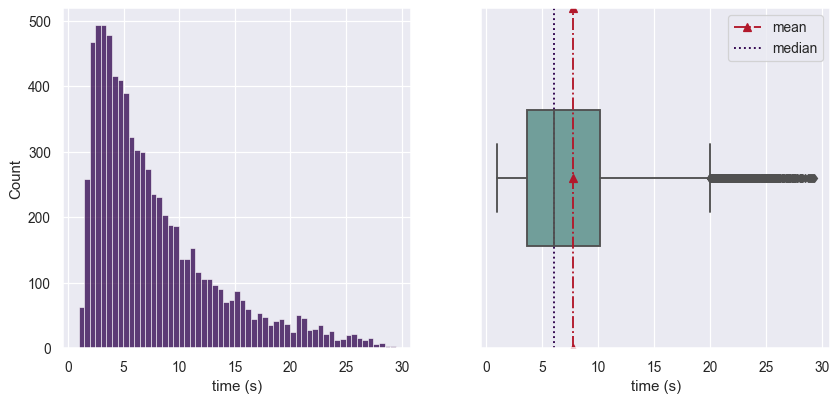
\includegraphics[width=150mm]{figures/RT_hist_box_23.png}
		\caption[Distribution of reaction times]{distribution of the  reaction times in the pointing task}
		\label{fig:rt_dists}
	\end{figure}
	
\end{enumerate}

\subsection{Extremes at starting locations}
In order to find out which of the 28 starting locations were the best and worst in performance with respect to the angular deviation from the target, the medians of angular deviation grouped by the starting locations were compared to the overall median of angular deviation.\\
As a result the starting location with the ID 9 which is a "patisserie" shop, therefore a context meaningful location, with the median of 19.18 degree deviation from the targets and the difference of 16.03 degree from the overall median (35.21) is the best location, i.e., has the lowest degree deviation from the target. See figure \ref{fig:best_angular}.\\
Furthermore, the starting location with the ID 35, one of the residential, thus not context meaningful, buildings with the angular deviation median of 52.49 degree away from the target and overall distance of 17.28 degree from the overall median (35.21) was the worst location of performing the task with regard to the angular deviation. See figure \ref{fig:worst_angular}.

\begin{figure}[h!]
	\centering
	\begin{subfigure}[b]{0.48\linewidth}
		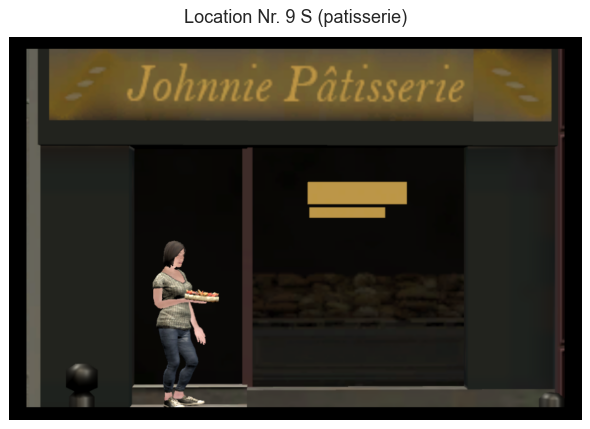
\includegraphics[width=\linewidth]{figures/best_loc_angular_error_withHA_23.png}
		\caption{best starting location}
		\label{fig:best_angular}
	\end{subfigure}
	\begin{subfigure}[b]{0.48\linewidth}
		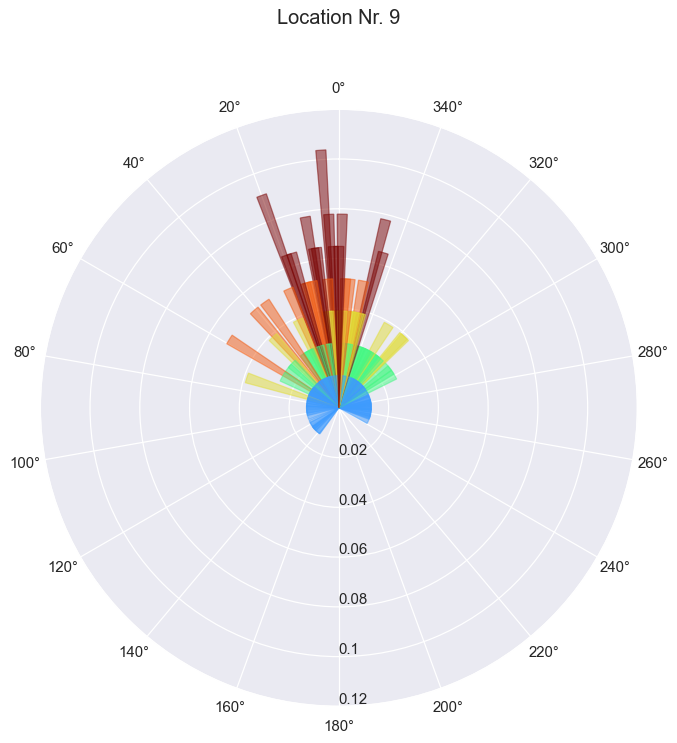
\includegraphics[width=\linewidth]{figures/deviation_degrees_loc_nr_9_23.png}
		\caption{angular deviation in location 9 (\%)}
		\label{fig:best_angular_dist_9}
	\end{subfigure}
	
	\caption[Best starting locations based on angular deviation]{the best starting location is chosen by taking the least median angular deviation among all starting locations.}
\end{figure}
\label{fig:best_location}

\begin{figure}[!h]
	\begin{subfigure}[b]{0.48\linewidth}
		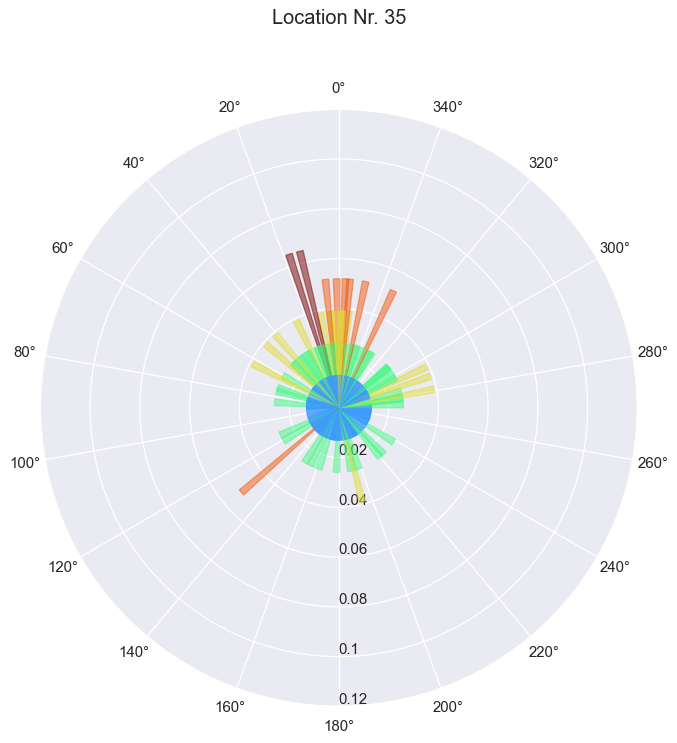
\includegraphics[width=\linewidth]{figures/deviation_degrees_loc_nr_35_23.png}
		\caption{angular deviation in location 35 (\%)}
		\label{fig:best_angular_dist_35}
	\end{subfigure}
	\begin{subfigure}[b]{0.48\linewidth}
		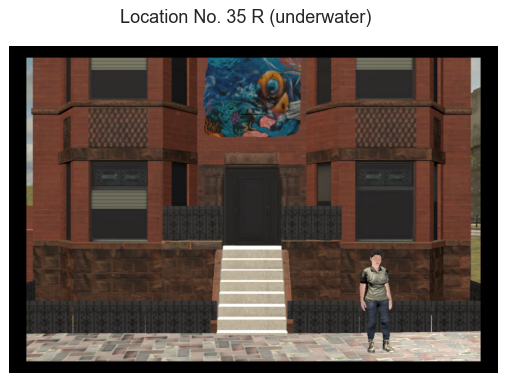
\includegraphics[width=\linewidth]{figures/worst_loc_angular_error__withHA_23.png}
		\caption{worst starting location}
		\label{fig:worst_angular}
	\end{subfigure}

	\caption[Worst starting location based on angular deviation]{the worst starting location is chosen by taking the highest median angular deviation among all starting locations.}
\end{figure}
\label{fig:worst_location}

\begin{figure}[h]
	\centering
	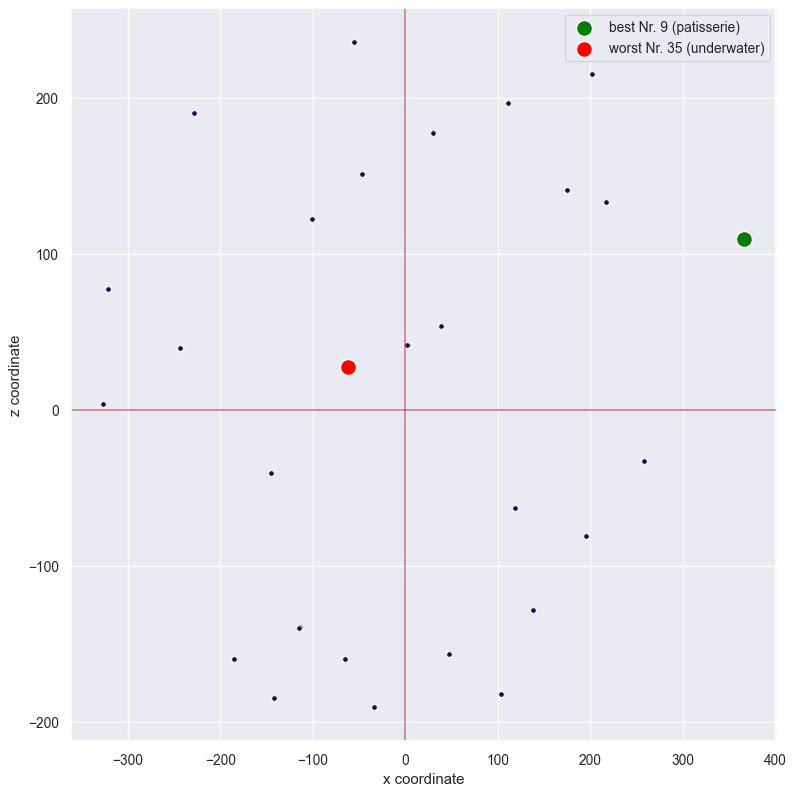
\includegraphics[width=100mm]{figures/best_worst_starting_locations.png}
	\caption[Locations of best and worst starting locations in city]{the locations of the best and worst starting locations inside the city coordinates.}
	\label{fig:best_worst_locs}
\end{figure}



\subsection{Linear mixed effects model (absolute angular error)}


\todo{
	- descriptive \\
	- assumption check \\
	- analysis results \\
	- exploratory analysis
	- add figures
}